\documentclass[crop, tikz]{standalone}
\makeatletter

\begin{document}

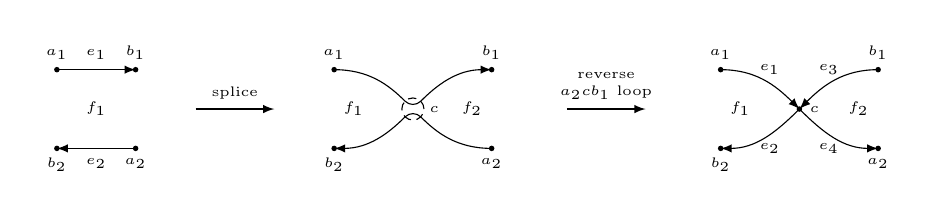
\begin{tikzpicture}[> = latex, font = \tiny]

\def\Q{20}

\matrix[column sep = 0.5 cm]{

	\draw [->] (-0.5, 0.5) -- node [above] {$e_1$} (0.5, 0.5);
	\draw [->] (0.5, -0.5) -- node [below] {$e_2$} (-0.5, -0.5);
	
	\fill (-0.5, 0.5) circle (1 pt) node [above] {$a_1$};
	\fill (0.5, 0.5) circle (1 pt) node [above] {$b_1$};
	
	\fill (0.5, -0.5) circle (1 pt) node [below] {$a_2$};
	\fill (-0.5, -0.5) circle (1 pt) node [below] {$b_2$};
	
	\node at (0, 0) {$f_1$};
	
	&
	
	\draw [->] (0, 0) -- node [above] {splice} (1, 0);
	
	&
	
	\fill (-1, 0.5) circle (1 pt) node [above] {$a_1$};
	\fill (1, 0.5) circle (1 pt) node [above] {$b_1$};
	
	\fill (1, -0.5) circle (1 pt) node [below] {$a_2$};
	\fill (-1, -0.5) circle (1 pt) node [below] {$b_2$};
	
	\draw [densely dashed] (0, 0) circle (4 pt) node [right = 0.25 em] {$c$};
	
	\draw [->, rounded corners] (-1, 0.5) to [out = 0, in = 135] (0, 0) to [out = 45, in = 180] (1, 0.5);
	\draw [->, rounded corners] (1, -0.5) to [out = 180, in = 315] (0, 0) to [out = 225, in = 0] (-1, -0.5);
	
	\node at (-0.75, 0) {$f_1$};
	\node at (0.75, 0) {$f_2$};
	
	&
	
	\draw [->] (0, 0) -- node [above, align = center] {reverse\\$a_2 c b_1$ loop} (1, 0);
	
	&
	
	\fill (-1, 0.5) circle (1 pt) node [above] {$a_1$};
	\fill (1, 0.5) circle (1 pt) node [above] {$b_1$};
	
	\fill (1, -0.5) circle (1 pt) node [below] {$a_2$};
	\fill (-1, -0.5) circle (1 pt) node [below] {$b_2$};
	
	\fill (0, 0) circle (1 pt) node [right = 0.25] {$c$};
	
	\draw [->] (-1, 0.5) to [out = 0, in = 135] (0, 0);
	\draw [->] (0, 0) to [out = 315, in = 180] (1, -0.5);
	
	\draw [->] (1, 0.5) to [out = 180, in = 45] (0, 0);
	\draw [->] (0, 0) to [out = 225, in = 0] (-1, -0.5);
	
	\node at (-0.375, 0.5) {$e_1$};
	\node at (-0.375, -0.5) {$e_2$};
	\node at (0.375, 0.5) {$e_3$};
	\node at (0.375, -0.5) {$e_4$};
	
	\node at (-0.75, 0) {$f_1$};
	\node at (0.75, 0) {$f_2$};

	\\
};

\end{tikzpicture}

\end{document}